\documentclass[a4paper,10pt,ngerman]{scrartcl}
\usepackage{babel}
\usepackage[T1]{fontenc}
\usepackage[utf8x]{inputenc}
\usepackage[a4paper,margin=2.5cm,footskip=0.5cm]{geometry}

% Die nächsten vier Felder bitte anpassen:
\newcommand{\Titel}{Schweinßnaht} % Aufgabennummer und Aufgabennamen angeben                      % Team-ID aus dem PMS angeben
\newcommand{\Name}{Adrian Surojit Müller\\ Daniel König\\ Karl Matti Schütz}                 % Team-Namen angeben          % Namen der Bearbeiter/-innen dieser Aufgabe angeben

%%% HEADERS & FOOTERS
\usepackage{fancyhdr, lastpage} % This should be set AFTER setting up the page geometry
\pagestyle{fancy} % options: empty , plain , fancy
\renewcommand{\headrulewidth}{1pt} % customise the layout...
\lhead{Seminarfacharbeit am ASG-Spez}
\chead{\Titel}
\rhead{\tiny\Name}
\lfoot{}
\cfoot{\thepage/\pageref{LastPage}}
\rfoot{}

% Position des Titels
\usepackage{titling}
\setlength{\droptitle}{-1.0cm}

% Für mathematische Befehle und Symbole
\usepackage{amsmath}
\usepackage{amssymb}

% Für Bilder
\usepackage{graphicx}

% Für Algorithmen
\usepackage{algpseudocode}

\usepackage{tikz}
\usepackage{float}
\usetikzlibrary{quotes,angles,arrows, calc, intersections}

% Für Quelltext
\usepackage{listings}
\usepackage{color}
\definecolor{mygreen}{rgb}{0,0.6,0}
\definecolor{mygray}{rgb}{0.5,0.5,0.5}
\definecolor{mymauve}{rgb}{0.58,0,0.82}
\lstset{
  keywordstyle=\color{blue},commentstyle=\color{mygreen},
  stringstyle=\color{mymauve},rulecolor=\color{black},
  basicstyle=\footnotesize\ttfamily,numberstyle=\tiny\color{mygray},
  captionpos=b, % sets the caption-position to bottom
  keepspaces=true, % keeps spaces in text
  numbers=left, numbersep=5pt, showspaces=false,showstringspaces=true,
  showtabs=false, stepnumber=2, tabsize=2, title=\lstname
}
\lstdefinelanguage{JavaScript}{ % JavaScript ist als einzige Sprache noch nicht vordefiniert
  keywords={break, case, catch, continue, debugger, default, delete, do, else, finally, for, function, if, in, instanceof, new, return, switch, this, throw, try, typeof, var, void, while, with},
  morecomment=[l]{//},
  morecomment=[s]{/*}{*/},
  morestring=[b]',
  morestring=[b]",
  sensitive=true
}

% Diese beiden Pakete müssen zuletzt geladen werden
%\usepackage{hyperref} % Anklickbare Links im Dokument
\usepackage{url}
\usepackage{hyperref}
\usepackage{cleveref}

\newcommand{\arrow}{$\rightarrow$ \ }
\newcommand{\hook}{$\hookrightarrow$ \ }
\newcommand{\botharrow}{$\Leftrightarrow $ \ }

\newcommand{\zitat}[1]{\glqq#1\grqq}
\renewcommand{\subitem}[1]{
    \begin{itemize}
        \item[\hook] #1
    \end{itemize}
}

% Daten für die Titelseite
\title{\vspace{2cm}\textbf{\Huge\Titel}\vspace{2cm}}
\author{
    \centering
    \large
    \begin{tabular}{ll}
        Verfasser: & Adrian Surojit Müller \\
            & Daniel König \\
            & Karl Matti Schütz \\ \\
        Seminarfachlehrer: & Frau Doktor Marion Moor \\ \\
        Fachlehrer: & Herr Bodo Gramsch \\ \\
        Außenbetreuer: & Herr Doktor Florian Römer \\ \\
        Einrichtung: & Spezialschulteil des Albert-Schweizer-Gymnasiums Erfurt \\ \\
        Datum der Abgabe: & \today 
    \end{tabular}
}
\date{}

\begin{document}

\begin{figure}
  \centering
  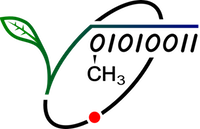
\includegraphics[scale=3]{img/logo.png}
\end{figure}
\maketitle

\newpage
\tableofcontents

\newpage
\textbf{Ideen}
\begin{itemize}
  \item B-Scan mit möglichen Fehlern abbilden
\end{itemize}

\newpage
\section{Entwicklung eines Programmes zur Fehlerbestimmung}
Anhand der vorherigen Kapitel sollte die Problematik der Fehlerbestimmung in Schweißnähten aufgefallen sein. 
Durch heutige technische Möglichkeiten, wäre dabei ein Schritt in Richting Digitalisierung dieses Verfahrens möglich. 
Dabei soll der Prüfer dennoch manuell einen Prüfkörper durch Ultraschall untersuchen, wobei die ermittelten Messdaten 
in einen Computer eingebettet werden sollen. \\ \\
Auf Grundlage der Datenformate an der Technischen Universiät Ilmenau (kurz TU Ilmenau), welche die ersten Daten bereitstellte, fiel die Wahl der Abspeicherung auf txt-Dateien. 
Dabei soll eine große Anzahl an Dateien erstellt werden, wobei jede einzelne Datei für einen bestimmten Punkt auf der Oberfläche 
der Schweißnaht steht. Desweiteren steht jede Zeile für einen bestimmten Zeitpunkt seit dem Beginn der Messung an diesem Punkt. 
Die Zeile ansich enthält einen gesampelten Wert für den Amplitudenausschlag. Dabei stehen meist um die 6000 Dateien 
mit je 1020 Werten zur Verfügung, wodurch eins der Hauptprobleme in der Programmentwicklung auffällig wird, 
denn diese Masse an Daten muss sowohl sinnvoll abgespeichert werden als auch möglichst schnell bearbeitet werden können. \\ \\
Die Wahl der Programmiersprache fiel dabei auf Python, da diese sehr einfach gehalten ist und bei den Mitgliedern der Gruppe bekannt ist, 
sowie auch im Bereich der Materialprüfung an der TU Ilmenau verwendet wird. 
Außerdem werden viel Bibliotheken (Erweiterungen) genutzt, wozu unter anderem Numpy zählt. Diese Bibliothek ergänzt Arrays, welche 
eine große Menge an Daten speichern können und schnellen Zugriff ermöglichen. Diese Numpy-Arrays können zusätzlich als NPY-Datei abgespeichert werden, 
welche sehr schnell ausgelesen werden können. Damit ist es möglich erworbene Messdaten in ein solches Array einzuordnen und im zugehörigen 
Dateiformat abzuspeichern, um wiederverwendbare Ergebnisse zu erhalten ohne die durch eine Messung entstehenden txt-Dateien in jeder Programmnutzung erneut auszuwerten. \\ \\
Zum besseren Verständnis der Daten, sollen jene in Diagrammen angezeigt werden, damit die errechneten Fehler mit den Schallrückgaben verglichen werden können. 
Dabei wurden die in Kapitel erwähnten A- und B-Scans implementiert, da diese deutliche Prognosen auf mögliche Fehler geben. 
Die Scans sind dabei in ihrem jeweiligen Reiter im Menu des Programms zu finden (eventuell Abbildung). 
Doch sollen die Fehler der Schweißnaht zusätzlich abbgebildet werden. Dabei wird eine Schweißnaht skizzenhaft
ausgegeben, wobei diese vereinfachte Darstellung auch von Experten dieses Themengebiets verwendet wird. 
An der sogennanten Nahtflanke\footnote{Schräge der Schweißnaht, welche Verbindung von Material zu Schweißmittel darstellt} sollen Fehler (siehe Kapitel) 
in Form von Kreisen eingezeichnet werden. Die Größe dieser Kreise ist dabei vorerst unbedeutend, da durch das gewählte und mit der 
TU Ilmenau entwickelte Verfahren keine Bestimmung dieser möglich ist. \\ \\
Die Bestimmung der Fehlerpositionen verläuft dabei über trigonometrische Berechnungen. Hierbei sind verschiedene Parameter zu berücksichtigen. 
Zum einen sind physikalische Merkmale wie Höhe oder der Winkel zum Lot (meist 45°) zu beachten, zum anderen 
sind jedoch die Messwerte entscheidend, wobei hier die Zeit heraussticht. Mithilfe der vergangenen Zeit, welche über die Position eines Messwertes in einer 
Datei ermittelt werden kann, lässt sich auf den zurückgelegten Weg des Ultraschalls schließen. Befindet sich an einer Stelle 
der Datei nun ein größerer Ausschlag der Amplitude, sollte an dieser Stelle ein Lufteinschluss vorhanden sein, 
welcher dann eingezeichnet wird. Da diese Makierung der Flankenbindefehler in einem 2D-Bild erfolgt, 
kann jeder mögliche Amplitudenausschlag überprüft werden, wodurch auch jede einzelne Zeile einer Datei überprüft werden muss. 
Dies ist mit viel Rechenaufwandt verbunden, was allerdings eine höhere Genauigkeit in diesem von Genauigkeit geprägten Milieu verspricht, 
denn wie in (Kapitel) zu lesen ist, kann jeder Fehler einer Naht verherrend sein. In der Anwendung ist die Berechnung dennoch 
sehr schnell, wodurch das Ziel einer Anwendung ohne lange Rechenzeiten nicht verfehlt wurde. \\ \\
\begin{figure}[H]
  \centering
  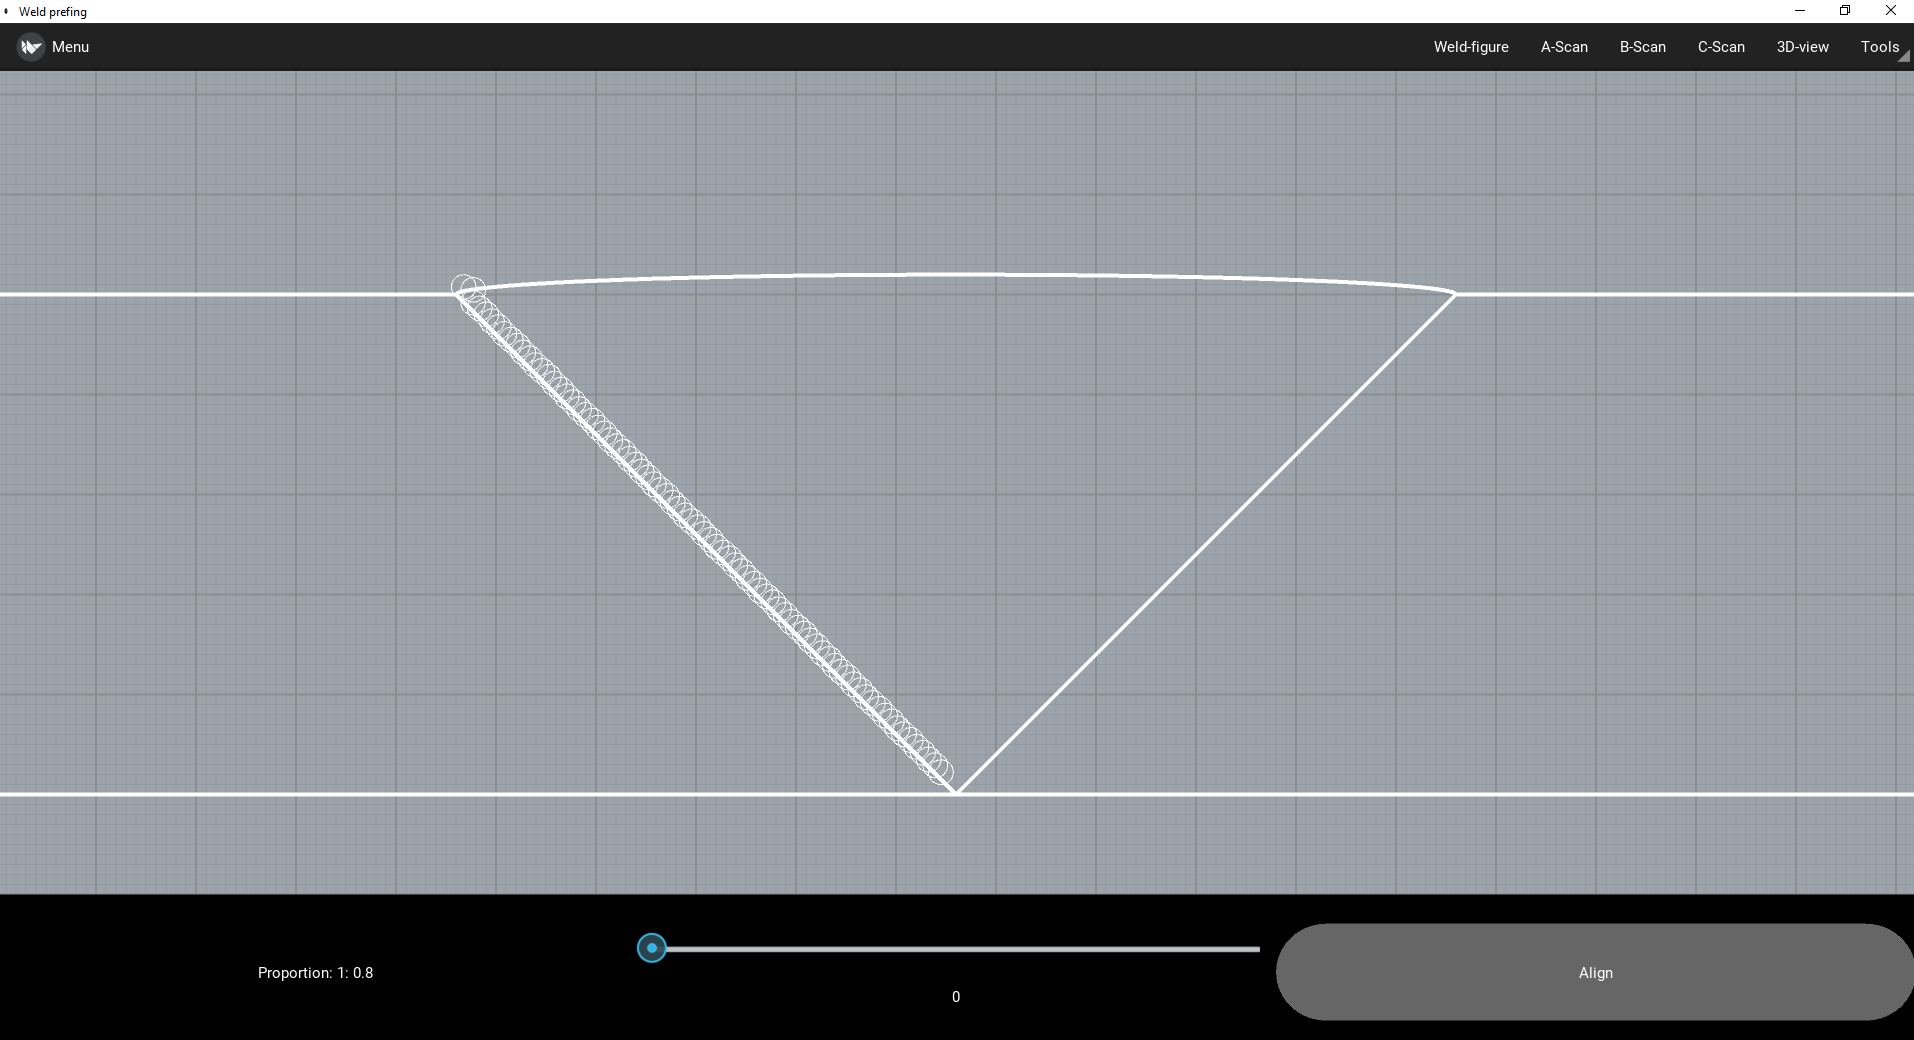
\includegraphics[width=\textwidth]{img/naht_fehlerlos.png}
  \caption{Eine simulierte Fehlerlose Schweißnaht}
\end{figure}
 


\newpage
\section*{Anhang}
\textbf{Bestimmung des Einschallwinkels zur Datenerhebung} \\
\begin{figure}[H]
\begin{tikzpicture}
  \pgfmathsetmacro{\x}{15};
  \pgfmathsetmacro{\y}{4};
  \pgfmathsetmacro{\angle}{22.5};

  \node[draw, circle] (A) at (0, \y) {A};
  \node[draw, circle] (C) at (\x, 0) {C};
  \node[draw, circle] (D) at (0, 0) {D};
  \node (H) at (\x, \y) {};

  \path (C)--++(\angle+90:5cm) coordinate (a);

  \node[draw, circle] (B) at (intersection of A--H and C--a) {B};

  \node[draw, circle] (E) at ($(B)!0.68!(C)$) {E};
  \node (b) at ($(E)!5cm!90:(C)$) {};

  \node[draw, circle] (M) at (intersection of E--b and D--C) {M};

  \path (M)--++(180-\angle:10cm) coordinate (c);
  \node[draw, circle] (Z) at (intersection of M--c and A--B) {Z};

  \path (Z)--++(0, -\y) coordinate (c);
  \node[draw, circle] (L) at (c) {L};

  %\draw (M) -- (last);

  \draw (A) -- (D) -- (L) -- (M) -- (C) -- (E) -- (B) -- (Z) -- (A);
  \draw[dashed] (C) -- (H) -- (B);
  \draw[color=green] (Z) -- (M) -- (E);

  \draw[dashed] (Z) -- (L);

  \pic [pic text=$\alpha$, draw, <->, angle radius=3cm] {angle = H--C--B};
  \pic [pic text=$\beta$, draw, <->, angle radius=1cm] {angle = B--C--D};

  \pic [pic text=$90\text{°}$, draw, <->, angle radius=2cm] {angle = B--E--M};
  \pic [pic text=$\alpha$, draw, <->, angle radius=2cm] {angle = C--M--E};
  \pic [pic text=$\alpha$, draw, <->, angle radius=2cm] {angle = A--M--D};

  \pic [pic text=$90\text{°}$, draw, <->, angle radius=1.5cm] {angle = M--L--Z};
  \pic [pic text=$\beta$, draw, <->, angle radius=1.5cm] {angle = L--Z--M};
\end{tikzpicture}
  \caption{Typische Skizze eines Schweißnahtmodells}
\end{figure}
\begin{align*}
  &\text{Durch den Nebenbwinkelsatz: } &\beta = 90\text{°}-\alpha \\ \\
  &\text{Für } \triangle EMC \text{ ist die Innenwinkelsumme 180°: } &\angle EMC+\beta+90\text{°} = 180\text{°} \\
  &&\angle EMC = 180\text{°} - 90\text{°} - \beta \\
  &\text{Mit } \beta=90\text{°}-\alpha \text{:}&\angle EMC = 90\text{°}-90\text{°}+\alpha \\
  && \angle EMC = \alpha \\ \\
  &\text{Da Einfallswinkel $=$ Ausfallwinkel:} & \angle LMZ=\angle EMC=\alpha \\ \\
  &\text{Für } \triangle ZML \text{ ist die Innenwinkelsumme 180°: } &\alpha+\angle LZM+90\text{°} = 180\text{°} \\
  && \angle LZM = 180\text{°} - \alpha - 90\text{°} \\
  && \angle LZM = 90\text{°} - \alpha=\beta
\end{align*}
Die grünen Strecken stehen sinnbildlich für den zurückgelegten Weg des Schalls, welcher sich 
strahlenförmig ausbreitet (Annahme aus dem Verfahren). Bei der Skizze steht die Strecke $\overline{ZL}$ 
für die Höhe $h$ eines Prüfkörpers, wobei für die Strecke $\overline{ZM}$, welche den Weg des Schalls bis 
zu der Reflektion am Boden meint, folgendes gilt: \\
\begin{align*}
  \overline{ZM} = \frac{\overline{ZL}}{\sin(\alpha)} = \frac{h}{\sin(\alpha)}
\end{align*}
\end{document}
